With a goal of recreating findings of O'Niel et al. \cite{lruk} we evaluated LRU-1, LRU-2 and LRU-3 algorithms on three workloads:
\begin{itemize}
\item a synthetic workload simulating alternating references to two pool pages with different frequencies,
\item a synthetic workload simulating random accesses according to Zipfian 80-20 distribution, and
\item buffer accesses captured with instrumentalized PostgreSQL running \texttt{pgbench}.
\end{itemize}

We present results for these workloads in the following sections.

\subsection{Two Pool Experiment}

As our first experiment, we replicated two pool experiment conducted by O'Niel et al. \cite{lruk}. They considered two pools of pages, Pool 1 with size $N_1$ and Pool 2 with $N_2$ pages and simulated random alternating accesses to those pools. With $N_1 << N_2$, the goal of this experiment was to simulate alternating accesses to index and record pages. Specifically, on every even access they uniformly choose one page from Pool 1 and on every odd access they choose one page from Pool 2. Thus, every page from Pool 1 has probability of reference $\frac{1}{2N_1}$ and every page from Pool 2 $\frac{1}{2N_2}$.

We replicated the experiment exactly, using $N_1 = 100$ and $N_2 = 10000$ pages. Figure \ref{fig:two_pool} shows measured hit rates for specific buffer sizes. Our results are consistent with O'Niel et al. \cite{lruk}, where they found that LRU-1 has lower hit rates than LRU-2 and LRU-3 for specific buffer size. We also see that LRU-1 performance approaches LRU-2 and LRU-3 on higher buffer sizes. LRU-2 and LRU-3 performances are similar, with LRU-3 slightly outperforming LRU-2. However, O'Niel et al. argues that the difference is too small to be traded for slower responsiveness that LRU-3 exhibits on evolving and dynamic access patterns.

\begin{figure}[t!]
    \centering
	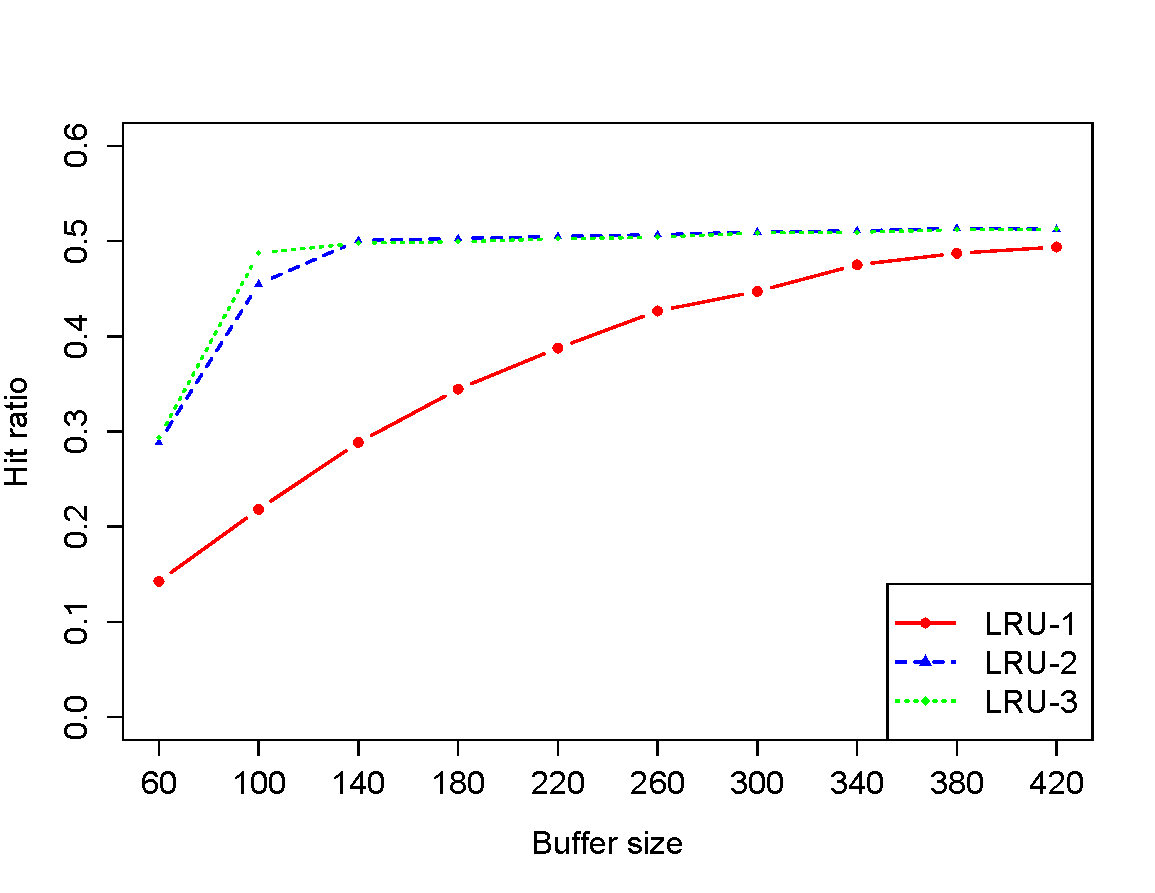
\includegraphics[width=0.5\textwidth]{./figures/two_pool.pdf}
	\caption{Simulation results of two pool experiment with disk page pools of $N_1 = 100$ pages and $N_2 = 10000$ pages. Horizontal axis shows the simulate buffer size and vertical axis shows measured hit ratio. All measurements were evaluated with Correlated Reference Period set to 0.}
	\label{fig:two_pool}
\end{figure}


\subsection{Zipfian Random Access Experiment}

\begin{figure}[t!]
    \centering
	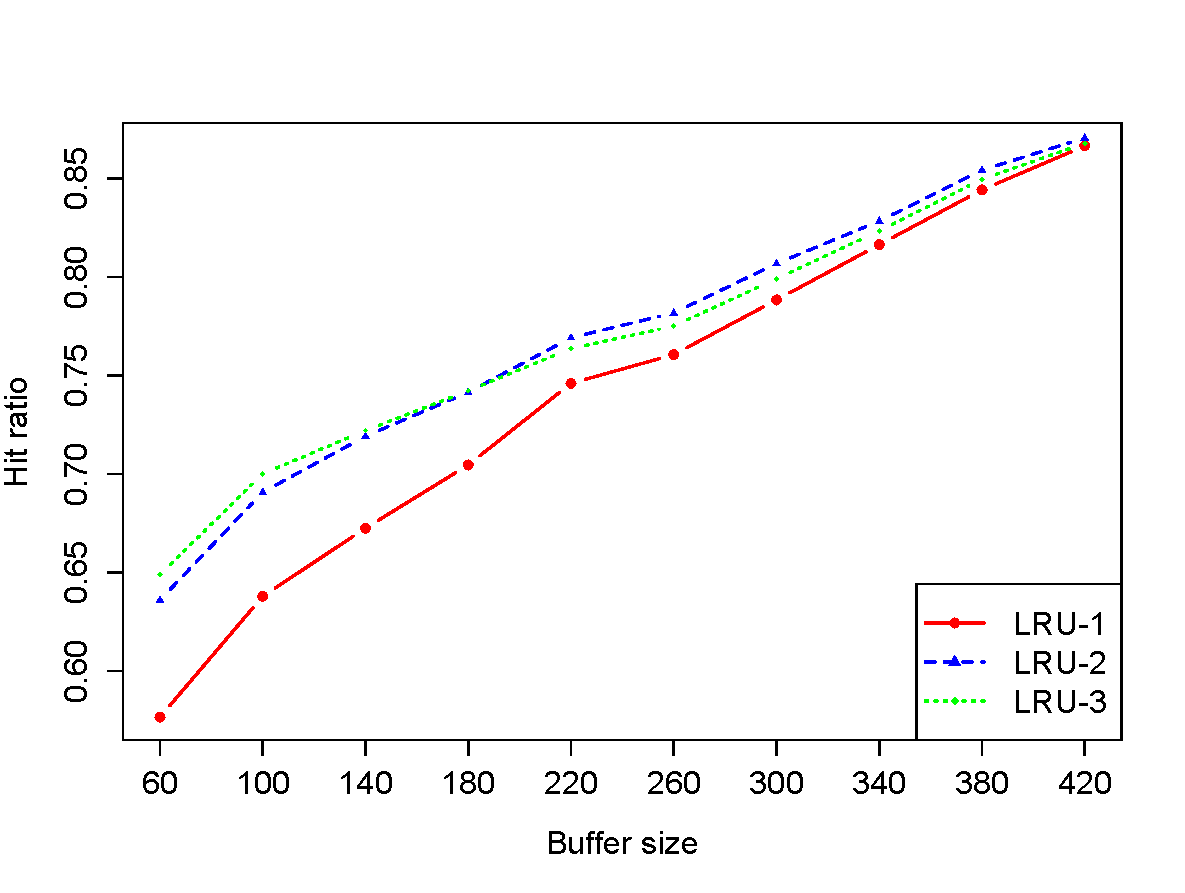
\includegraphics[width=0.5\textwidth]{./figures/zipfian.pdf}
	\caption{Simulation results of cache hit ratio for random access with Zipfian 80-20 distribution to $N = 1000$ pages in the pool. Horizontal axis shows the simulate buffer size and vertical axis shows measured hit ratio. All measurements were evaluated with Correlated Reference Period set to 0.}
	\label{fig:zipfian}
\end{figure}


\subsection{PostgreSQL Trace Experiment}

\begin{figure}[t!]
    \centering
	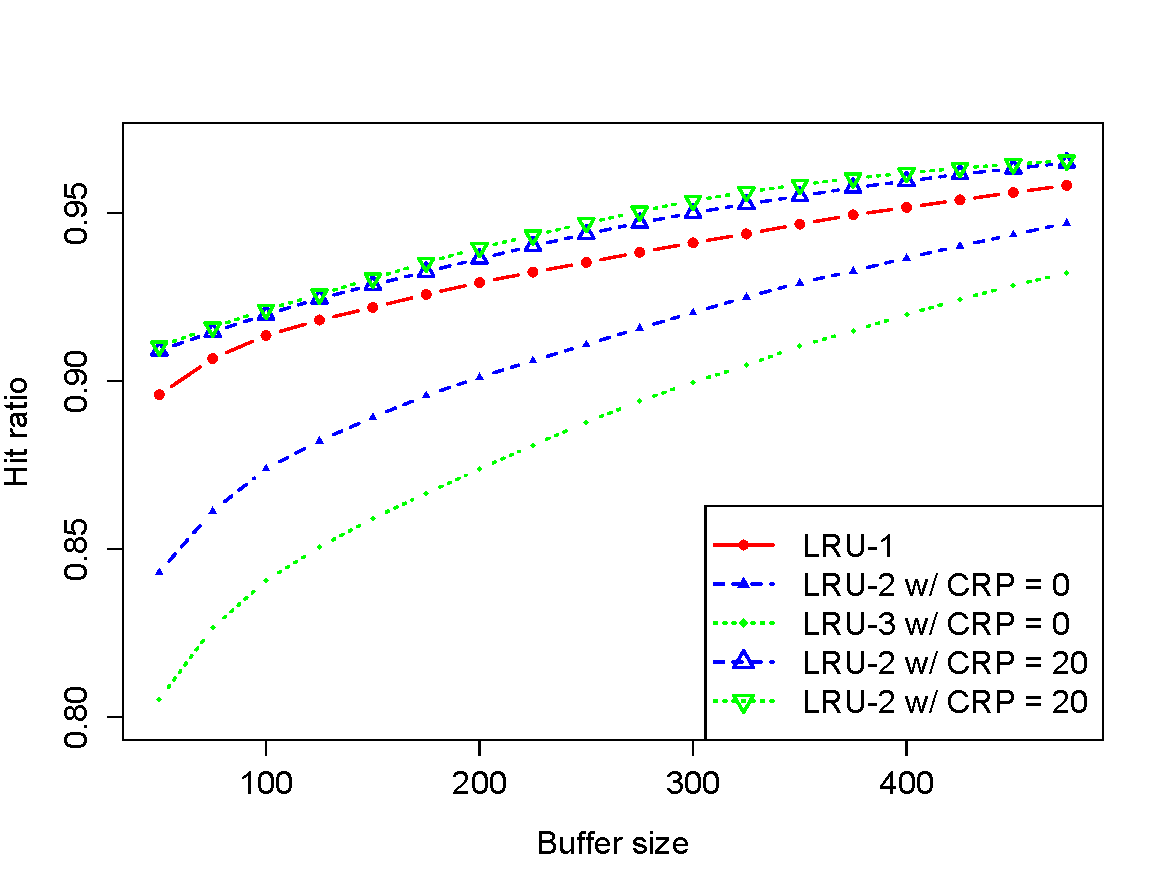
\includegraphics[width=0.5\textwidth]{./figures/postgres.pdf}
	\caption{Simulation results of different buffer management strategies using a trace collected from PostgreSQL running \texttt{pgbench} benchmark. Horizontal axis shows the simulate buffer size and vertical axis shows measured hit ratio. LRU-2 and LRU-3 are evaluated with Correlated Reference Period set to 0 and 20.}
\end{figure}
